
Os modelos matemáticos que descrevem o comportamento do ângulo de arfagem (\textit{pitch}), ângulo de guinada (\textit{yaw}), \textit{cross-pitch} e \textit{cross-yaw}, foram obtidos pelo método de identificação em malha aberta. Que consiste na aplicação de um sinal de excitação na planta e coleta e análise de sua resposta a essa entrada. O modelo matemático é então obtido relacionando-se o sinal de saída com o sinal de entrada por meio de um sistema padrão de 2ª ordem ou modificações dele.

Como se trata de um sistema MIMO, foi necessário identificar quatro FTs, a saber: a do ângulo de arfagem $G_{\Phi}$ (\textit{pitch}), a do ângulo de guinada $G_{\Psi}$ (\textit{yaw}), a do \textit{cross-pitch} $G_{cp}$ e a do \textit{cross-yaw} $G_{cy}$. A representação do sistema em diagrama de blocos é mostrada na Figura \ref{fig:IdentificaMIMOSystem}.

\begin{figure}[H]
    \centering
    \includegraphics[width=0.48\textwidth]{figures/Identificacao/Identificacao_MIMO.pdf}
    \caption{Diagrama de blocos do sistema MIMO.}
    \label{fig:IdentificaMIMOSystem}
\end{figure}

\noindent onde $U_{1}(s)$ e $U_{2}(s)$ representam as tensões aplicadas nos motores que controlam os rotores do \textit{pitch} e do \textit{yaw}, e $\Phi(s)$ e $\Psi(s)$ os ângulos de arfagem e de guinada, respectivamente.

%%%%%%%%%%%%%%%%%%%%%%%%%%%%%%%%%%%%%%%%%%%%%%%%%%%%%%%%%%%%%
\subsection{\textbf{Modelagem do ângulo de arfagem (\textit{pitch})}}

Para identificar o modelo do ângulo de arfagem, foram aplicados dois degraus, um de amplitude $\SI{1.36}{\volt}$ e outro de amplitude $\SI{0.34}{\volt}$. A soma dessas amplitudes corresponde à tensão que deixa o rotor paralelo ao chão. A resposta do ângulo do rotor a essa entrada é mostrada na Figura \ref{fig:IdentificacaoPitchAngle}.

\begin{figure}[H]
    \centering
    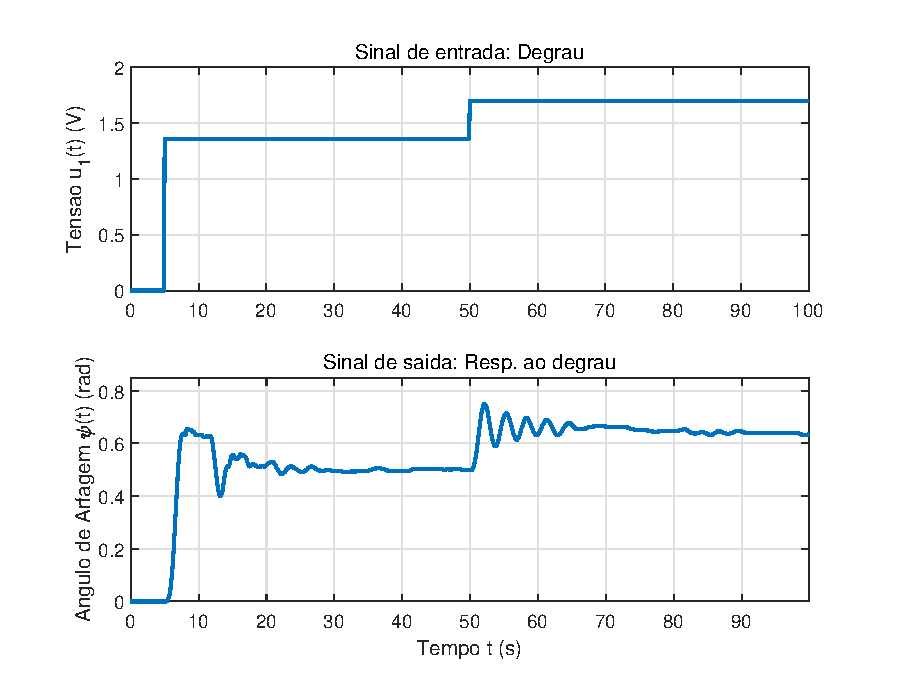
\includegraphics[width=0.48\textwidth]{figures/Identificacao/IdentificaPitchInicial.eps}
    \caption{Identificação do modelo do ângulo de arfagem (\textit{pitch}).}
    \label{fig:IdentificacaoPitchAngle}
\end{figure}

Para a identificação do modelo, apenas a resposta ao segundo degrau foi considerada. Pois, para variações de baixa amplitude, o sistema não sai do entorno de seu ponto de operação e responde, portanto, de forma linear. 

A resposta obtida é típica de um sistema padrão de segunda ordem subamortecido $( 0 < \zeta \leq 1)$. Considerando a existência de tempo-morto, a função de transferência de interesse é da forma
\begin{equation}\label{eq:FTPitch}
    G_{\psi}(s) = \frac{\Psi(s)}{U_{1}(s)} = \frac{k w_{n}^2 e^{-\tau_d s}}{s^2 + 2 \zeta w_{n} s + w_{n}^2}
\end{equation}
\noindent onde $k$ é o ganho estático, $w_n$ a frequência natural de oscilação (em $\si{\radian/\s}$), $\zeta$ é o coeficiente de amortecimento e $\tau_d$ o tempo-morto em $\si{s}$.

Com $t_{i}$ e $t_{i+1}$ os instantes de tempo em que ocorrem dois picos consecutivos na resposta, a frequência amortecida pode ser aproximada por
$$ w_d = \frac{2 \pi}{T} \approx \frac{2 \pi}{t_{i+1} - t_i} = \frac{2 \pi}{30.2 - 27.1} = \SI{2.0268}{\radian/\s} $$
\noindent já um valor inicial para $\zeta$, de acordo com \cite{aguirre2004}, pode ser obtido contando-se o número $N$ de picos visíveis na resposta
$$ \zeta \approx \frac{0.6}{N} = \frac{0.6}{5} = 0.12 $$
\noindent e o ganho estático
$$ k = \frac{\Delta \psi}{\Delta u_{1}} = \frac{0.7486 - 0.7148}{0.34} = 0.0994 $$
Após sobrepor as respostas da planta e do modelo, removendo a condição inicial (deslocado para a origem), tal como mostrado na Figura \ref{fig:IdentificacaoPitchAngleDesloc}, os valores do coeficiente de amortecimento e do ganho foram ajustados para
$$ \zeta = 0.06 \quad\text{e}\quad k = 0.462 $$
e para esse novo valor de $\zeta$, obteve-se
$$ w_{n} = \frac{w_{d}}{\sqrt{1 - \zeta^2}} = \SI{2.03049}{\radian/\s} $$
O valor do atraso foi obtido por inspeção: $\tau_{d} \approx \SI{0.5}{\s}$.

\begin{figure}[H]
    \centering
    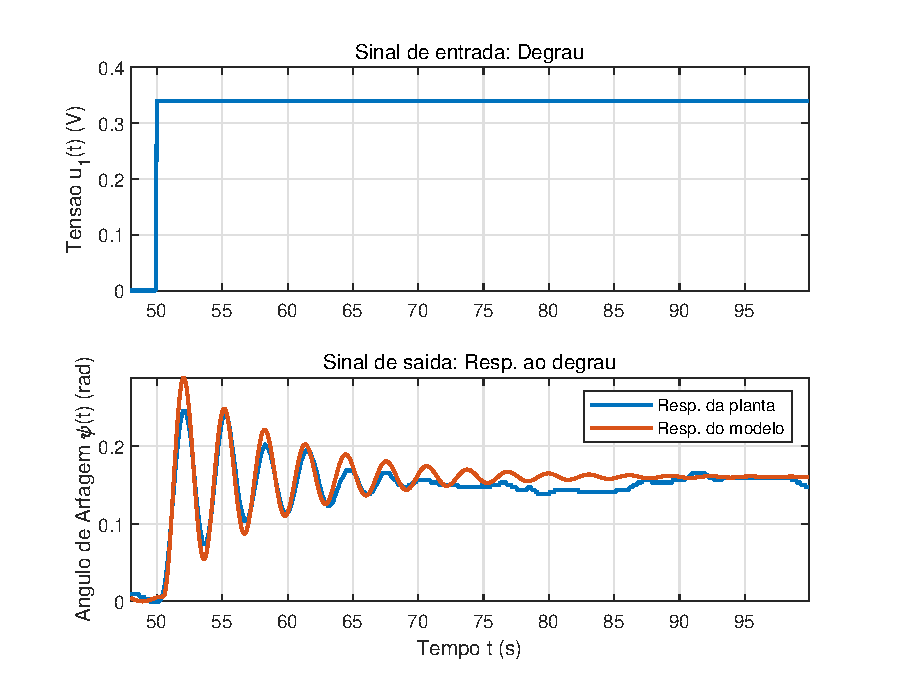
\includegraphics[width=0.48\textwidth]{figures/Identificacao/IdentificaPitchFinal.eps}
    \caption{Sinal original e modelo identificado para o ângulo de arfagem (\textit{pitch}).}
    \label{fig:IdentificacaoPitchAngleDesloc}
\end{figure}

Assim, o modelo matemático que descreve o comportamento do ângulo de arfagem é dado por
\begin{equation}\label{eq:FTModeloIDPitch}
    G_{\psi}(s) = \frac{\Psi(s)}{U_{1}(s)} = \frac{1.905 e^{-0.5 s}}{s^2 + 0.2437 s + 4.123}
\end{equation}

%%%%%%%%%%%%%%%%%%%%%%%%%%%%%%%%%%%%%%%%%%%%%%%%%%%%%%%%%%%%%%%%%%%%%%%%%%%%%%%%%%%
%%%%%%%%%%%%%%%%%%%%%%%%%%%%%%%%%%%%%%%%%%%%%%%%%%%%%%%%%%%%%%%%%%%%%%%%%%%%%%%%%%%
%%%%%%%%%%%%%%%%%%%%%%%%%%%%%%%%%%%%%%%%%%%%%%%%%%%%%%%%%%%%%%%%%%%%%%%%%%%%%%%%%%%
\subsection{\textbf{Modelagem do ângulo de guinada (\textit{yaw})}}

Para identificar o modelo do ângulo de guinada, foi aplicado um degrau de amplitude $\SI{0.6}{\volt}$. Um valor baixo de tensão foi necessário devido a excursão limitada da rotação do eixo do rotor da cauda, impedindo que se chegasse ao fim de curso e prejudicasse a qualidade do sinal medido do ângulo. A resposta do ângulo do rotor da cauda a essa entrada é mostrada na Figura \ref{fig:IdentificacaoYawAngleInicial}.

\begin{figure}[H]
    \centering
    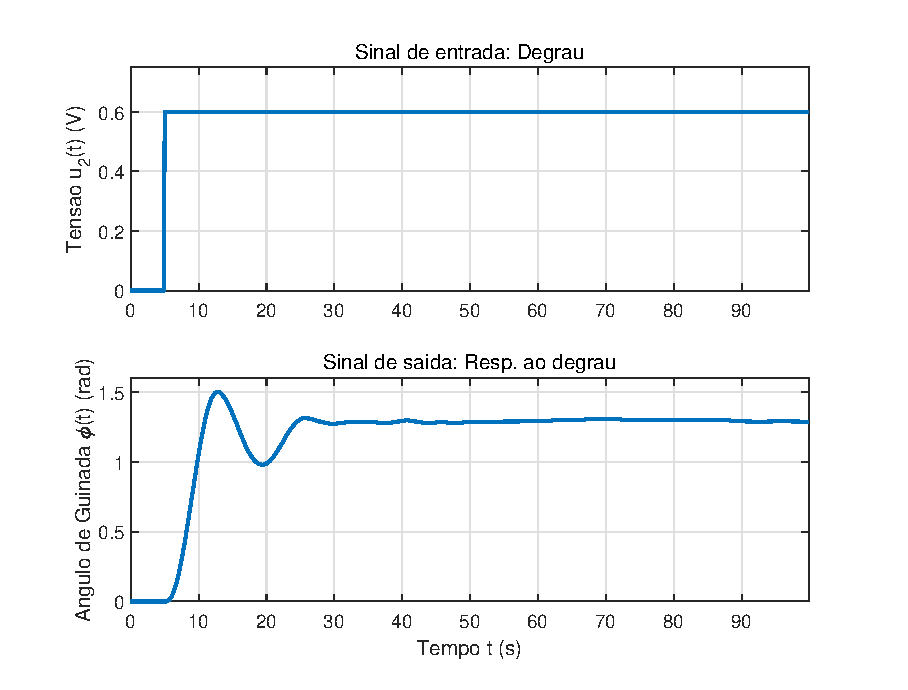
\includegraphics[width=0.48\textwidth]{figures/Identificacao/IdentificaYawInicial.eps}
    \caption{Identificação do modelo do ângulo de guinada (\textit{yaw}).}
    \label{fig:IdentificacaoYawAngleInicial}
\end{figure}

A resposta obtida é, novamente, típica de um sistema padrão de segunda ordem subamortecido $( 0 < \zeta \leq 1)$. Considerando a existência de tempo-morto, a função de transferência de interesse é da forma
\begin{equation}\label{eq:FTYaw}
    G_{\phi}(s) = \frac{\Phi(s)}{U_{2}(s)} = \frac{k w_{n}^2 e^{-\tau_d s}}{s^2 + 2 \zeta w_{n} s + w_{n}^2}
\end{equation}
\noindent onde $k$ é o ganho estático, $w_n$ a frequência natural de oscilação (em $\si{\radian/\s}$), $\zeta$ é o coeficiente de amortecimento e $\tau_d$ o tempo-morto em $\si{s}$.

Com $t_{i}$ e $t_{i+1}$ os instantes de tempo em que ocorrem dois picos consecutivos no ângulo de guinada, a frequência amortecida foi aproximada por
$$ w_d = \frac{2 \pi}{T} \approx \frac{2 \pi}{t_{i+1} - t_i} = \frac{2 \pi}{25.5-12.8} = \SI{0.5026}{\radian/\s} $$
\noindent o valor inicial para $\zeta$, \cite{aguirre2004}, foi obtido a partir do número $N$ de picos visíveis no sinal de saída
$$ \zeta \approx \frac{0.6}{N} = \frac{0.6}{2} = 0.3 $$
\noindent já o ganho estático
$$ k = \frac{\Delta \phi}{\Delta u_{2}} = \frac{1.5 - 1.285}{0.6} = 0.3583 $$
Esses parâmetros foram então ajustados por meio da sobreposição das respostas da planta e do modelo, a fim de se obter um melhor ajuste. Os valores finais para $\zeta$, $w_{n}$, $k$ foram
$$ \zeta = 0.42 \quad\text{e}\quad k = 1.65 \quad\text{e}\quad w_{n} = \SI{0.47}{\radian/\s} $$
O valor do atraso, obtido por inspeção, foi $\tau_{d} \approx \SI{0.5}{\s}$.

Assim, o modelo matemático que descreve o comportamento do ângulo de guinada é dado por
\begin{equation}\label{eq:FTModeloIDYaw}
    G_{\phi}(s) = \frac{\Phi(s)}{U_{2}(s)} = \frac{0.3645 e^{-0.5 s}}{s^2 + 0.3948s + 0.2209}
\end{equation}
O resultado da sobreposição do modelo identificado com o sinal original do ângulo de guinada é mostrado na Figura \ref{fig:IdentificacaoYawAngleFinal}.

\begin{figure}[H]
    \centering
    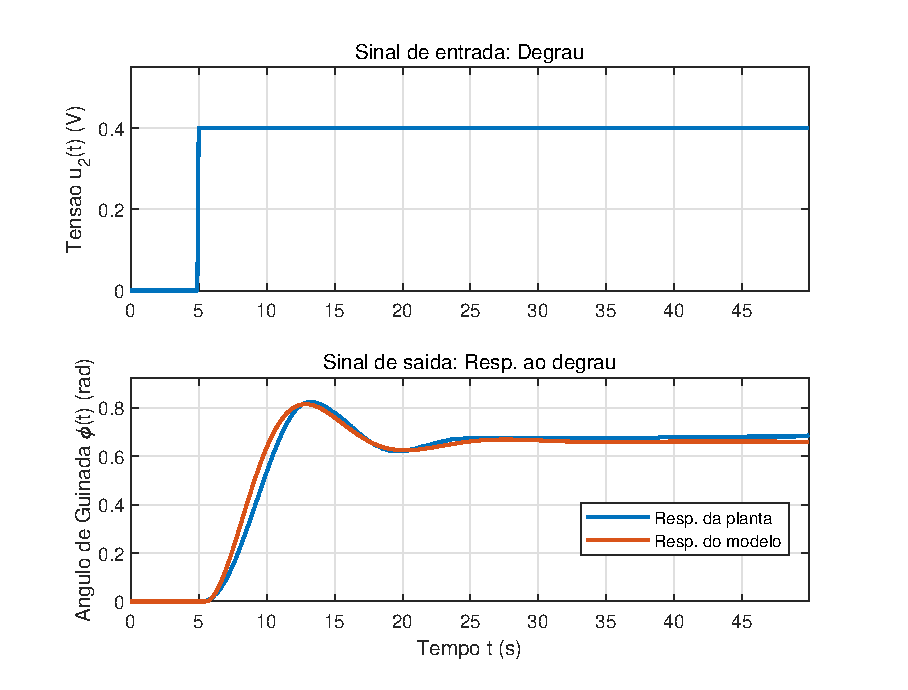
\includegraphics[width=0.48\textwidth]{figures/Identificacao/IdentificaYawFinal.eps}
    \caption{Sinal original e modelo identificado para o ângulo de guinada (\textit{yaw}).}
    \label{fig:IdentificacaoYawAngleFinal}
\end{figure}

%%%%%%%%%%%%%%%%%%%%%%%%%%%%%%%%%%%%%%%%%%%%%%%%%%%%%%%%%%%%%%%%%%%%%%%%%%%%%%%%%%%
%%%%%%%%%%%%%%%%%%%%%%%%%%%%%%%%%%%%%%%%%%%%%%%%%%%%%%%%%%%%%%%%%%%%%%%%%%%%%%%%%%%
%%%%%%%%%%%%%%%%%%%%%%%%%%%%%%%%%%%%%%%%%%%%%%%%%%%%%%%%%%%%%%%%%%%%%%%%%%%%%%%%%%%
\subsection{\textbf{Modelagem do \textit{cross-pitch}}}

Para identificação do modelo do \textit{cross-pitch}, que relaciona a tensão aplicada no rotor dianteiro (principal) com a variação do ângulo de guinada (\textit{yaw}), foi aplicada uma tensão em $u_{1}$ (rotor dianteiro), na forma de um degrau de amplitude $\SI{1}{\volt}$. Esse sinal de entrada e a resposta do ângulo \textit{yaw}, para $u_{2} = 0$, tensão no rotor da cauda nula, são mostradas na Figura \ref{fig:IdentificacaoCrossPitchInicial}.

\begin{figure}[H]
    \centering
    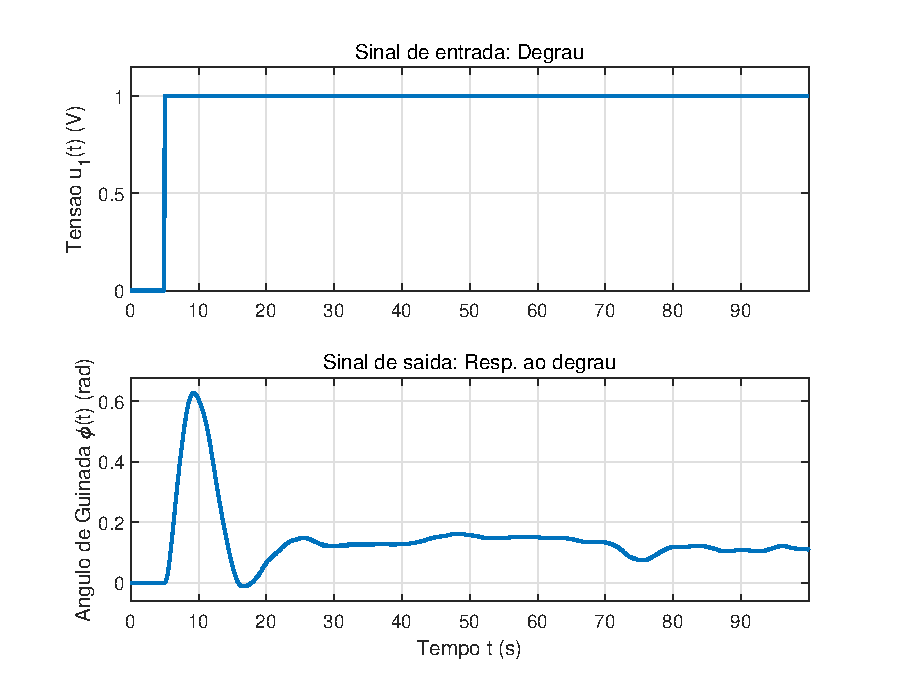
\includegraphics[width=0.48\textwidth]{figures/Identificacao/IdentificaCrossPitchInicial.eps}
    \caption{Identificação do modelo do \textit{cross-pitch}.}
    \label{fig:IdentificacaoCrossPitchInicial}
\end{figure}

Para relacionar esses sinais, buscou-se identificar um modelo da forma
\begin{equation}\label{eq:FTCrossPitch}
    G_{cp}(s) = \frac{\Phi(s)}{U_{1}(s)} = \frac{k w_{n}^2 (a_{1} s + a_{0})e^{-\tau_d s}}{s^2 + 2 \zeta w_{n} s + w_{n}^2}
\end{equation}
\noindent onde $k$ é o ganho estático, $w_n$ a frequência natural de oscilação (em $\si{\radian/\s}$), $\zeta$ é o coeficiente de amortecimento, $\tau_d$ o tempo-morto em $\si{s}$ e $a_{1}$ e $a_{0}$ são os coeficientes do numerador.

Para tanto, foi utilizada a ferramenta de identificação \textit{Ident} do \textit{Matlab}. A partir dos sinais de entrada e saída fornecidos, obteve-se o seguinte modelo para a FT do \textit{cross-pitch}
\begin{equation}\label{eq:FTModeloIDCrossPitch}
    G_{cp}(s) = \frac{\Phi(s)}{U_{1}(s)} = \frac{0.3025(s+0.06162)e^{-s}}{s^2 + 0.2574 s + 0.1437}
\end{equation}
O resultado da sobreposição do modelo identificado na equação \eqref{eq:FTModeloIDCrossPitch} com o sinal original do \textit{cross-pitch} é mostrado na Figura \ref{fig:IdentificacaoCrossPitchFinal}.

\begin{figure}[H]
    \centering
    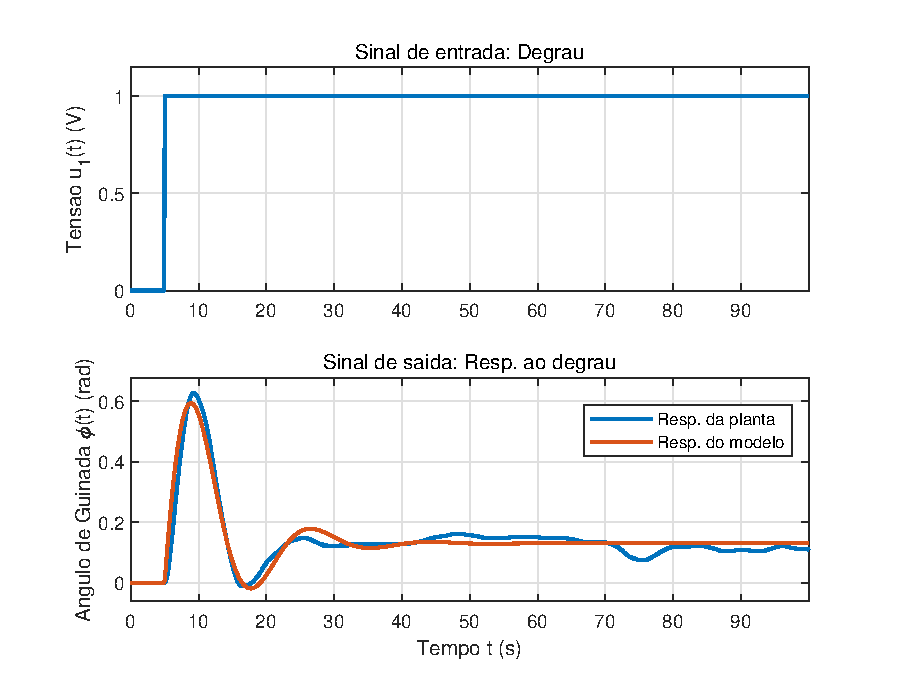
\includegraphics[width=0.48\textwidth]{figures/Identificacao/IdentificaCrossPitchFinal.eps}
    \caption{Sinal original e modelo identificado para o \textit{cross-pitch}.}
    \label{fig:IdentificacaoCrossPitchFinal}
\end{figure}

%%%%%%%%%%%%%%%%%%%%%%%%%%%%%%%%%%%%%%%%%%%%%%%%%%%%%%%%%%%%%%%%%%%%%%%%%%%%%%%%%%%
%%%%%%%%%%%%%%%%%%%%%%%%%%%%%%%%%%%%%%%%%%%%%%%%%%%%%%%%%%%%%%%%%%%%%%%%%%%%%%%%%%%
%%%%%%%%%%%%%%%%%%%%%%%%%%%%%%%%%%%%%%%%%%%%%%%%%%%%%%%%%%%%%%%%%%%%%%%%%%%%%%%%%%%
\subsection{\textbf{Modelagem do \textit{cross-yaw}}}

Já a identificação do modelo do \textit{cross-yaw}, que busca relacionar a tensão aplicada no rotor da cauda com a variação do ângulo de arfagem (\textit{pitch}), se valeu da aplicação de uma tensão em $u_{2}$ (rotor da cauda), na forma de um degrau com amplitude $\SI{0.6}{\volt}$. A Figura \ref{fig:IdentificacaoCrossYawInicial} mostra o sinal de entrada da tensão aplicada e a resposta do ângulo \textit{pitch} para essa entrada, com $u_{1} = 0$, tensão no rotor dianteiro nula.

\begin{figure}[H]
    \centering
    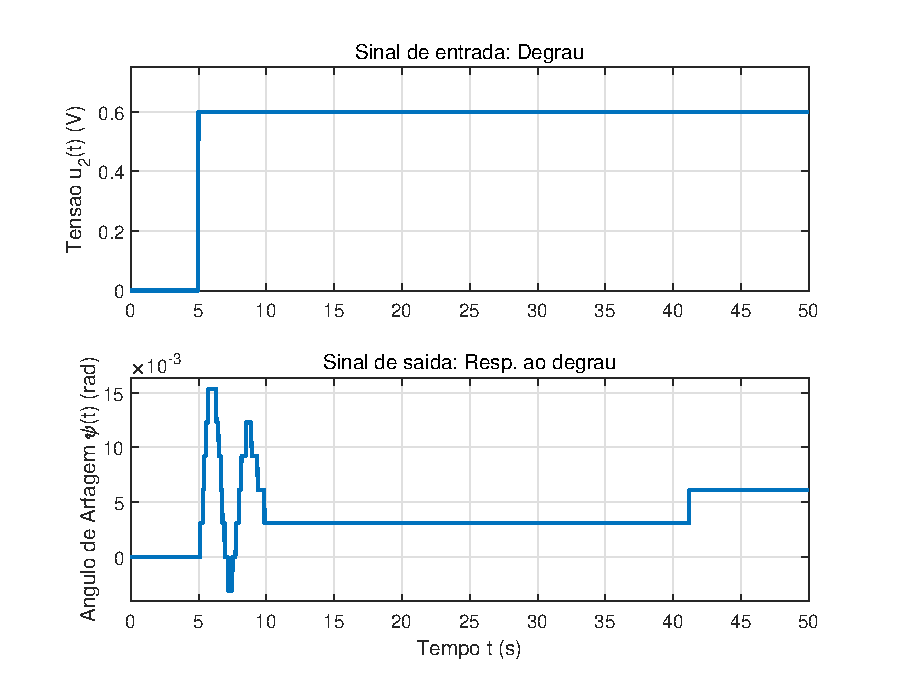
\includegraphics[width=0.48\textwidth]{figures/Identificacao/IdentificaCrossYawInicial.eps}
    \caption{Identificação do modelo do \textit{cross-yaw}.}
    \label{fig:IdentificacaoCrossYawInicial}
\end{figure}

O modelo utilizado para relacionar esses sinais foi da forma
\begin{equation}\label{eq:FTCrossYaw}
    G_{cy}(s) = \frac{\Psi(s)}{U_{2}(s)} = \frac{k w_{n}^2 (a_{1} s + a_{0})e^{-\tau_d s}}{s^2 + 2 \zeta w_{n} s + w_{n}^2}
\end{equation}
\noindent onde $k$ é o ganho estático, $w_n$ a frequência natural de oscilação (em $\si{\radian/\s}$), $\zeta$ é o coeficiente de amortecimento, $\tau_d$ o tempo-morto em $\si{s}$ e $a_{1}$ e $a_{0}$ são os coeficientes do numerador.

Utilizando-se novamente a ferramenta de identificação do \textit{Matlab}, obteve-se o seguinte modelo para a FT do \textit{cross-yaw}, para os sinais de entrada e saída fornecidos
\begin{equation}\label{eq:FTModeloIDCrossYaw}
    G_{cy}(s) = \frac{\Psi(s)}{U_{2}(s)} = \frac{0.0476(s+1.2945)e^{-0.13s}}{s^2 + 0.6339 s + 4.262}
\end{equation}
A Figura \ref{fig:IdentificacaoCrossYawFinal} mostra o resultado da sobreposição do modelo identificado na equação \eqref{eq:FTModeloIDCrossYaw} com o sinal original do \textit{cross-yaw}.

\begin{figure}[H]
    \centering
    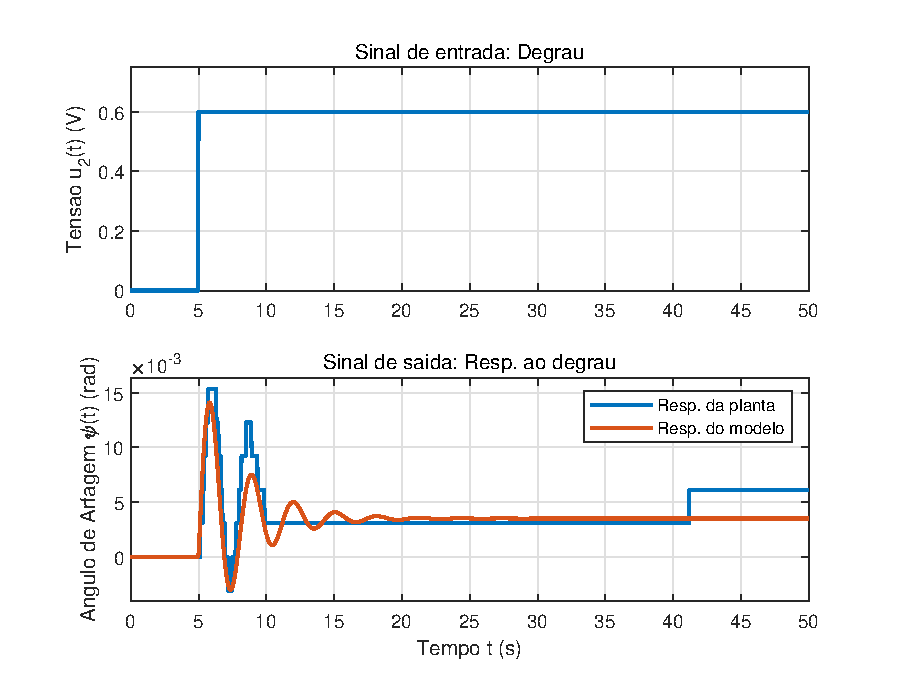
\includegraphics[width=0.48\textwidth]{figures/Identificacao/IdentificaCrossYawFinal.eps}
    \caption{Sinal original e modelo identificado para o \textit{cross-yaw}.}
    \label{fig:IdentificacaoCrossYawFinal}
\end{figure}

%%%%%%%%%%%%%%%%%%%%%%%%%%%%%%%%%%%%%%%%%%%%%%%%%%%%%%%%%%%%%%%%%%%%%%%%%%%%%%%%%%%
%%%%%%%%%%%%%%%%%%%%%%%%%%%%%%%%%%%%%%%%%%%%%%%%%%%%%%%%%%%%%%%%%%%%%%%%%%%%%%%%%%%
%%%%%%%%%%%%%%%%%%%%%%%%%%%%%%%%%%%%%%%%%%%%%%%%%%%%%%%%%%%%%%%%%%%%%%%%%%%%%%%%%%%
\subsection{\textbf{Modelos Identificados}}

Um resumo das FTs identificadas para os ângulos de arfagem, guinada, além do \textit{cross-pitch} e \textit{cross-yaw}, respectivamente, são mostradas nas equações a seguir:

\begin{equation}\tag{\ref{eq:FTModeloIDPitch}}
    G_{\psi}(s) = \frac{\Psi(s)}{U_{1}(s)} = \frac{1.905 e^{-0.5 s}}{s^2 + 0.2437 s + 4.123}
\end{equation}

\begin{equation}\tag{\ref{eq:FTModeloIDYaw}}
    G_{\phi}(s) = \frac{\Phi(s)}{U_{2}(s)} = \frac{0.3645 e^{-0.5 s}}{s^2 + 0.3948s + 0.2209}
\end{equation}

\begin{equation}\tag{\ref{eq:FTModeloIDCrossPitch}}
    G_{{cp}_{21}}(s) = \frac{\Phi(s)}{U_{1}(s)} = \frac{0.3025(s+0.06162)e^{-s}}{s^2 + 0.2574 s + 0.1437}
\end{equation}

\begin{equation}\tag{\ref{eq:FTModeloIDCrossYaw}}
    G_{{cy}_{12}}(s) = \frac{\Psi(s)}{U_{2}(s)} = \frac{0.0476(s+1.2945)e^{-0.13s}}{s^2 + 0.6339 s + 4.262}
\end{equation}

Na próxima seção esses modelos são validados para outros sinais de entrada, ou seja, sinais com características diferentes dos utilizados na fase de identificação.